%% Pass options to hyperref BEFORE oblivoir loads it internally
\PassOptionsToPackage{hidelinks}{hyperref}
\documentclass[a4paper,10pt]{oblivoir}

%% ----- 패키지 -----
\usepackage{amsmath,amssymb,amsfonts}
\usepackage{graphicx}
\usepackage{booktabs}
\usepackage{array}
%% hanging pkg removed (conflicts with oblivoir/memoir)
\usepackage{setspace}
%% hyperref already loaded by oblivoir -- do NOT reload it
\usepackage{geometry}
\usepackage{caption}
\usepackage{float}
\usepackage{tikz}
\usetikzlibrary{arrows.meta,shapes.geometric,positioning,calc}

\geometry{a4paper, top=25mm, bottom=25mm, left=25mm, right=25mm}
\setstretch{1.8}
\setcounter{secnumdepth}{0}   %% suppress auto section numbers (titles already numbered)
\setcounter{tocdepth}{0}
\graphicspath{{./}}
%% hangparas environment already provided by oblivoir (via hanging pkg loaded internally)
%% -- no need to define it here

\title{베이지안 부분점수모형 기반 구조방정식 모형(PCM-SEM)을 활용한\\
학문 목적 한국어 학습자의 쓰기 태도 연구:\\
주월랑(2022) 데이터 재분석 및 방법론적 비교}
\author{KOS-5101 시뮬레이션 연구}
\date{2026년 4월}

\begin{document}
\maketitle

\begin{abstract}
주월랑(2022)은 외국인 유학생 86명을 대상으로 21개 Likert 5점 척도 문항으로 쓰기 태도의 세 하위 구인—쓰기인식(X), 쓰기반응(M), 수행태도(Y)—을 측정하고 집단 간 차이를 분석하였다. 그러나 합산 점수(composite score)를 OLS 회귀에 투입하는 분석 방식은 문항 측정 오차로 인한 회귀 감쇠 편향(attenuation bias)을 내포하며, 구인 간 인과 경로와 매개 효과를 정밀하게 추정하지 못한다는 방법론적 한계가 있다. 본 연구는 이 한계를 부분 신용 모형(Partial Credit Model, PCM)과 구조 방정식 모형(SEM)을 통합한 베이지안 PCM-SEM으로 보완하는 방법론 연구이다.
원논문의 요약 통계(N=86, 구인별 복합 점수 평균)를 사전 분포의 근거로 활용하여 시뮬레이션 데이터를 생성하고, 약한 사전 분포(semi-informative) 모형과 원논문 기반 강한 사전 분포(informative) 모형을 Stan/NUTS-HMC로 추정하였다. \textbf{주요 결과}: (1) 쓰기인식\ensuremath{\rightarrow}쓰기반응 경로($\beta_1$)는 두 모형 모두에서 유의미한 양의 효과가 확인되었다; (2) 쓰기반응\ensuremath{\rightarrow}수행태도 경로($\beta_2$)는 강한 사전 분포 모형에서만 유의하여, 소표본에서 사전 정보가 추론의 질을 결정함을 보여준다; (3) 직접 효과($\gamma_1$)가 비유의하여 쓰기반응을 통한 완전 매개(full mediation) 구조가 지지된다; (4) 간접 효과 역시 강한 사전 분포 모형에서 유의하게 추정되었다; (5) 성별 효과는 두 모형 모두 비유의로 원논문 결과와 일치한다. 보충 몬테카를로 시뮬레이션은 합산 점수 OLS가 표본 크기에 무관한 체계적 편향을 내포하며, 표본이 커질수록 포함 확률이 명백히 저하됨을 확인하였다. 이상의 결과는 PCM-SEM이 원논문에서 검토되지 않은 인과 매개 구조를 규명하고 측정 오차 문제를 해소함을 보여준다.
\textbf{주제어}: 부분 신용 모형, 구조 방정식 모형, 베이지안 추론, 쓰기 태도, 매개 효과, 회귀 감쇠 편향, 몬테카를로 시뮬레이션
---
\end{abstract}
\section{1. 서론}

외국인 유학생의 한국어 쓰기 태도 연구(주월랑, 2022)는 21개 Likert 5점 척도 문항으로 세 하위 구인—쓰기인식(필요성\ensuremath{\cdot}가치 인식), 쓰기반응(흥미\ensuremath{\cdot}자신감), 수행태도(내용 생성\ensuremath{\cdot}조직\ensuremath{\cdot}고쳐쓰기 태도)—을 측정하고 학습자 요인(학년, 성별, 한국어 숙달도, 어학원 경험)에 따른 집단 차이를 분석하였다. 연구 결과, 대부분의 학습자 요인과 쓰기 태도 사이에 유의미한 차이가 없었으며, 이는 언어 숙달도와 정의적 쓰기 태도가 독립적으로 작동함을 시사하였다.

그러나 이 연구는 중요한 방법론적\ensuremath{\cdot}이론적 질문을 남긴다. 세 하위 구인은 개념적으로 위계적\ensuremath{\cdot}인과적 관계를 가질 수 있다. 쓰기에 대한 인지적 가치 인식(쓰기인식)은 정서적 반응(쓰기반응)을 예측하고, 이 정서적 반응이 다시 실제 수행 태도(수행태도)로 이어지는 경로는 태도 형성 이론(Ajzen \& Fishbein, 1977; Bandura, 1977)과 일치한다. 원논문은 이 인과 경로를 직접 검증하지 않았다.

방법론적으로는, 합산 점수를 OLS 회귀에 투입하는 방식이 문항 수준 측정 오차를 무시함으로써 경로 계수를 체계적으로 과소추정하는 회귀 감쇠 편향(Spearman, 1904; Fuller, 1987)의 문제를 안고 있다.

본 연구의 목적은 다음 세 가지이다. 첫째, 원논문의 요약 통계를 사전 정보로 활용하여 베이지안 PCM-SEM을 적용하고, 원논문이 검토하지 않은 쓰기 태도 구인 간 인과 매개 구조를 규명한다. 둘째, 약한 사전 분포와 강한 사전 분포(원논문 통계 기반) 모형을 비교하여 사전 정보의 영향을 평가한다. 셋째, 몬테카를로 시뮬레이션으로 합산 점수 OLS 대비 PCM-SEM의 통계적 우위를 정량화한다.

\subsubsection{1.1 시뮬레이션 기반 연구의 학술적 정당성}

원논문의 개별 응답 데이터가 공개되어 있지 않으므로, 본 연구는 원논문의 요약 통계(M, SD, n)를 바탕으로 시뮬레이션 데이터를 생성하여 분석한다. 이 접근법은 세 가지 근거로 학술적으로 정당하다.

\textbf{첫째, 베이지안 지식 누적(cumulative knowledge)의 원리.} 원논문의 결과를 직접 "재분석"하는 것이 아니라, 그 결과값들을 베이지안 모형의 정보적 사전 분포(informative priors)로 투입하여 지식을 누적하는 방식이다. "이전 연구의 원자료를 보지 못하더라도, 이전 연구가 확립한 효과 크기와 분포 특성을 사전 지식으로 삼아 새로운 분석을 수행한다"는 이 논리는 베이지안 추론의 핵심이며, 메타분석(Hedges \& Olkin, 1985)이나 순차 베이지안 학습(Bernardo \& Smith, 1994)과 동일한 인식론적 토대 위에 있다. 원논문의 하위 구인별 평균(X=4.015, M=3.348, Y=3.171), 표준편차, 그리고 보고된 상관계수(r(성별, X)=.290)가 사전 분포 하이퍼파라미터 설정에 직접 반영되었다는 점에서, 본 연구는 원논문 지식의 베이지안 갱신(Bayesian updating)으로 정당화된다.

\textbf{둘째, 반사실적 방법론 연구(counterfactual methodology).} 원논문의 측정 구조(21개 문항, 5점 척도, N=86)를 충실히 재현한 시뮬레이션은 "만약 원논문에서 PCM-SEM을 적용하였다면 어떤 결론이 가능하였는가"라는 반사실적 질문에 답한다. 이는 Muthén \& Muthén(2002)이 정립한 방법론 연구의 표준 설계이며, 새로운 분석 도구의 적용 가능성을 기존 연구 맥락에서 검증하는 독립적 학술 기여이다.

\textbf{셋째, 데이터 생성의 충실성.} 시뮬레이션이 학술적 타당성을 갖추려면 생성 데이터가 원논문의 통계적 특성을 충실히 반영해야 한다. 본 연구는 PCM 임계값 이분 탐색 보정, 원논문 성비(여성 68.6\%) 적용, 구인 간 상관 구조를 구조 방정식 파라미터로 인코딩하는 세 단계 절차를 통해 이를 달성하였다. 구체적 알고리즘은 3.1절에서 상술한다.


\section{2. 이론적 배경}

\subsubsection{2.1 쓰기 태도의 구조와 인과 경로}

본 연구는 외국인 유학생의 쓰기 태도를 단순한 단일 구인이 아닌, 인지적\ensuremath{\cdot}정서적\ensuremath{\cdot}행동적 요소가 유기적으로 연결된 위계적 구조로 상정한다. 이를 위해 심리학의 태도 구성 요소 모델인 \textbf{ABC 모델(Affect, Behavior, Cognition)}과 제2언어 습득 이론의 정의적 여과기(Affective Filter) 가설을 결합하여 다음과 같은 인과 경로를 설정하였다.

첫째, 쓰기인식(Cognition, $X$)은 글쓰기의 학술적 가치와 중요성에 대한 지적 판단을 의미하며, 이는 모든 태도 형성의 시발점이 된다. 그러나 인지적 자각이 곧바로 실제 수행으로 이어지기에는 심리적 간극이 존재한다.

둘째, 이 간극을 매개하는 변인으로서 쓰기반응(Affect, $M$)을 설정하였다. 쓰기반응은 글쓰기에 대한 즐거움, 자신감, 혹은 불안과 같은 정서적 차원을 포함한다. 인지적으로 글쓰기의 중요성을 수용($X$)하더라도, 학습자가 정서적으로 긍정적인 반응($M$)을 형성하지 못할 경우 행동의 변화로 나아가는 동력이 약화될 수 있다.

셋째, 최종 종속 변인인 수행태도(Behavior, $Y$)는 독자 고려, 고쳐쓰기 전략 사용 등 실제적인 쓰기 행동 의지를 나타낸다. 본 연구는 인지적 인식($X$)이 정서적 반응($M$)을 거칠 때 비로소 능동적인 수행태도($Y$)로 치환된다는 매개 경로 가설을 수립하였다.

\[ X(\text{쓰기인식}) \rightarrow M(\text{쓰기반응}) \rightarrow Y(\text{수행태도}) \]

이러한 위계적 경로는 주월랑(2022)의 연구에서 나타난 '숙달도와 태도 간의 낮은 상관관계'를 구조적으로 해명할 수 있는 틀을 제공한다. 즉, 유학생들의 숙달도가 높아짐에 따라 쓰기의 중요성에 대한 인식($X$)은 향상될 수 있으나, 정서적 반응($M$) 경로에서 병목 현상이 발생할 경우 실제 수행($Y$)의 변화로 이어지지 않을 가능성을 시사한다.

이 경로는 태도 형성의 표준적인 심리 프로세스와 일치한다. 심리학의 ABC 모델(Ajzen \& Fishbein, 1977)에서 인지($X$)가 정서($M$)를 변화시키고, 정서가 최종적인 행동 의도($Y$)를 이끌어낸다는 설명과 궤를 같이하며, 자기결정성 이론(Self-Determination Theory)의 관점에서도 내재적 동기 형성에 정의적 반응이 필수적 매개 역할을 담당한다(Bandura, 1977). 또한, 많은 유학생들이 한국어 쓰기가 중요함을 인지하고 있음에도 실제 수행 전략을 사용하지 않는 이유는, 그 과정에서 느끼는 불안(Anxiety)이나 흥미 결여(Low Interest)라는 정의적 병목에서 찾을 수 있으며, 본 연구의 매개 모형은 이 메커니즘을 구조적으로 규명한다.

또한, 성별($G$)을 외생 변수로 투입하여 이러한 심리적 경로의 기저 수준이 성별에 따라 차이가 있는지를 통제함으로써 모델의 설명력을 높이고자 하였다.

\subsubsection{2.2 부분 신용 모형 (PCM)}

Masters(1982)가 제안한 PCM은 순서형 다분 문항 반응에 대한 Rasch 계열 측정 모형이다. $K$개 범주를 가진 문항 $i$에서 개인 $j$의 응답이 범주 $k$일 로그-오즈는:

\[ \log \frac{P(X_{ij} = k \mid \theta_j)}{P(X_{ij} = k-1 \mid \theta_j)} = \theta_j - \delta_{ik} \]

여기서 $\theta_j$는 개인의 잠재 구인 수준, $\delta_{ik}$는 문항 $i$의 $k$번째 임계값(threshold)이다. 이 모형은 $\theta_j$와 $\delta_{ik}$의 분리성(separability)을 보장함으로써, 개인의 잠재 수준을 문항 특성으로부터 독립적으로 추정한다.

\subsubsection{2.3 PCM-SEM 통합 모형}

측정 방정식(PCM)과 구조 방정식(SEM)을 통합한 완전 베이지안 모형은 다음과 같다.

\textbf{측정 방정식}: 각 구인의 문항 응답이 해당 잠재 변수에서 PCM에 따라 생성된다.

\[ y_{ij} \sim \text{PCM}(\theta_j^{(c)}, \boldsymbol{\delta}_i), \quad c = X, M, Y \]

\textbf{구조 방정식} (잔차 분산 = 1 고정, 식별을 위함):

\[ \theta_j^{(M)} = \alpha_M + \beta_1 \theta_j^{(X)} + \gamma_M G_j + \varepsilon_M, \quad \varepsilon_M \sim \mathcal{N}(0, 1) \]
\[ \theta_j^{(Y)} = \alpha_Y + \gamma_1 \theta_j^{(X)} + \beta_2 \theta_j^{(M)} + \gamma_Y G_j + \varepsilon_Y, \quad \varepsilon_Y \sim \mathcal{N}(0, 1) \]

여기서 $G_j$는 성별 공변량이다.

\textbf{효과 분해}:

\[ \text{간접 효과} = \beta_1 \cdot \beta_2, \quad \text{직접 효과} = \gamma_1, \quad \text{총 효과} = \gamma_1 + \beta_1 \beta_2 \]

\textbf{식별 조건}: (1) $\theta^{(X)} \sim \mathcal{N}(0, 1)$ 사전 분포로 X의 척도\ensuremath{\cdot}위치 고정; (2) M\ensuremath{\cdot}Y의 잔차 표준편차 = 1 고정(척도 식별); (3) M\ensuremath{\cdot}Y 구인 임계값 합-영 제약(위치 식별).

\begin{figure}[htbp]
\centering
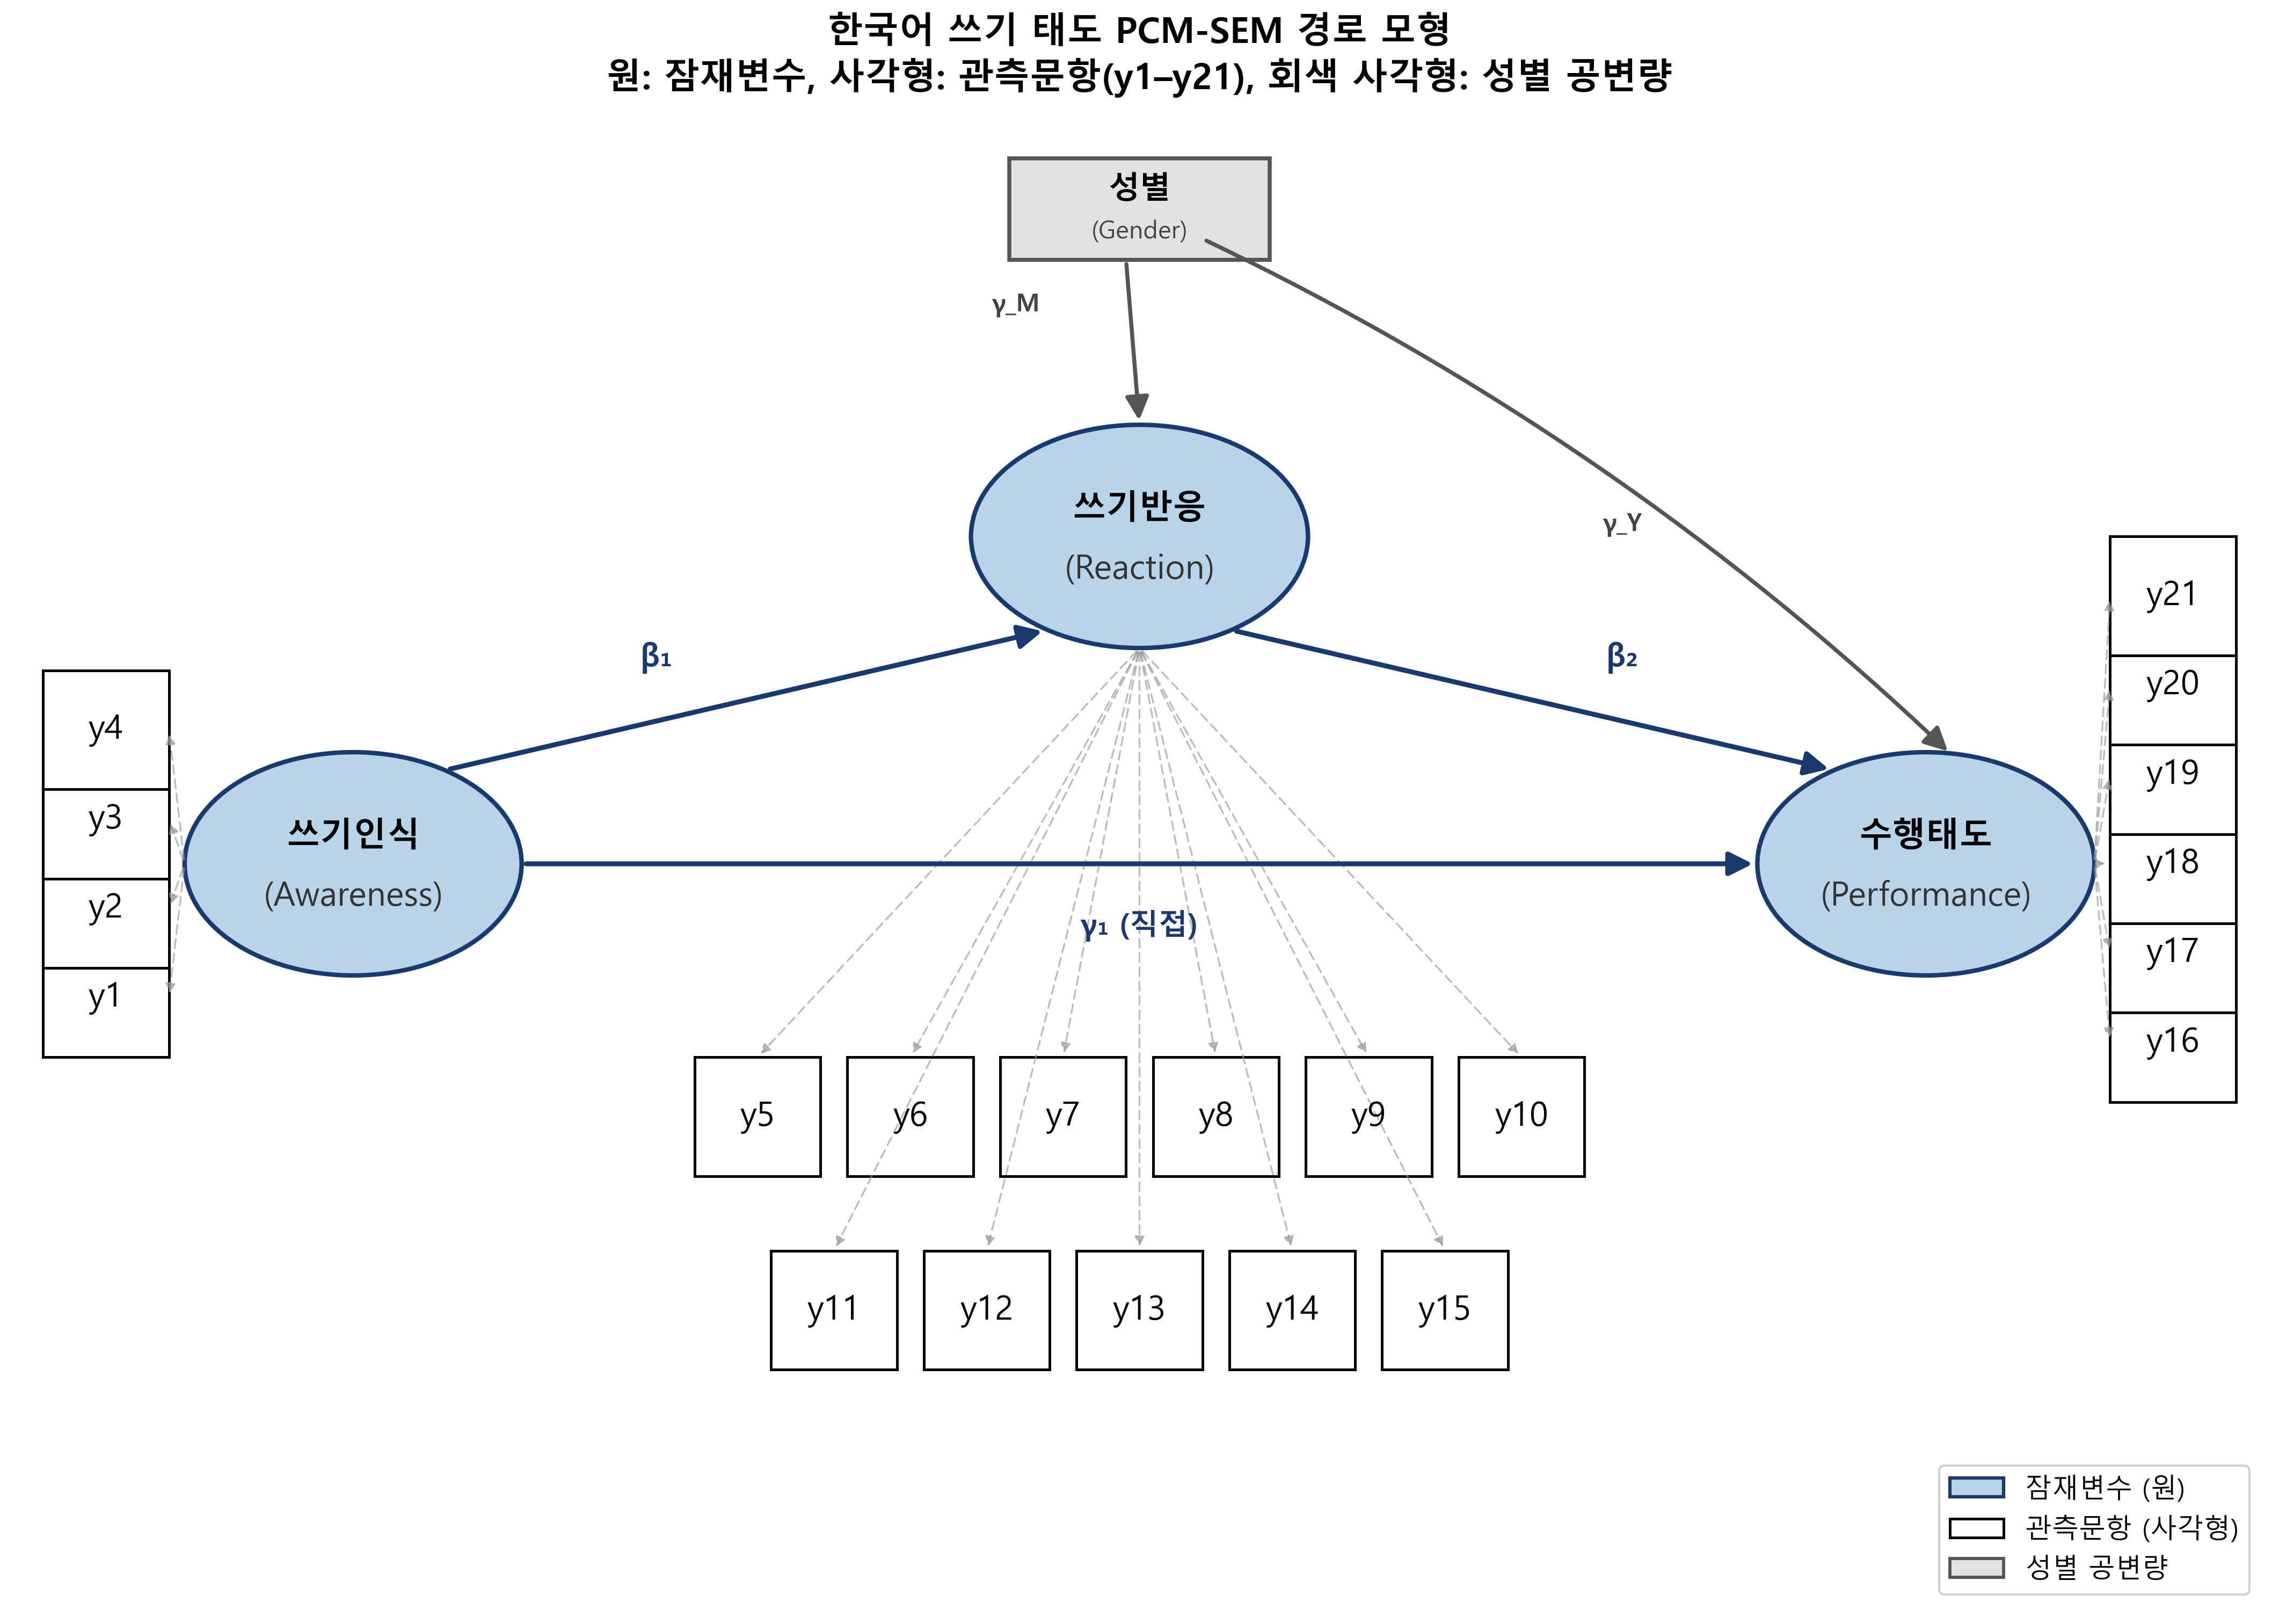
\includegraphics[width=0.8\textwidth]{sem_path_diagram_korean.png}
\caption{그림 1. 한국어 쓰기 태도 PCM-SEM 경로 모형. 원: 잠재 변수, 사각형: 관측 문항(y1–y21), 회색 사각형: 성별 공변량.}
\end{figure}

\subsubsection{2.4 회귀 감쇠 편향}

측정 오차를 포함한 합산 점수 $\hat{X} = X + e$를 OLS에 투입할 경우:

\[ E[\hat{\beta}_{1,\text{OLS}}] = \beta_1 \cdot \lambda_X, \quad \lambda_X = \frac{\text{Var}(X)}{\text{Var}(X) + \text{Var}(e)} < 1 \]

$\lambda_X$는 신뢰도 계수이다. 이 편향은 \textbf{표본 크기에 무관하게} 지속된다(불일관 추정). PCM-SEM은 잠재 변수 $\theta$를 직접 추정하므로 $\lambda = 1$이 되어 감쇠 편향이 발생하지 않는다.

\subsubsection{2.5 베이지안 추론의 이점}

베이지안 PCM-SEM은 빈도주의 방법 대비 다음의 추가 정보를 제공한다.

\textbf{인과 방향성 확률}: $P(\beta_1 > 0 \wedge \beta_2 > 0 \mid \text{data})$를 사후 분포에서 직접 계산하여, "두 경로가 모두 양의 방향인 확률"을 수량화한다.

\textbf{간접 효과의 완전한 사후 분포}: 빈도주의 델타법(Sobel, 1982)은 간접 효과에 대해 근사적 신뢰구간만 제공하지만, 베이지안 접근법은 $\beta_1\beta_2$의 완전한 사후 분포를 산출한다.

\textbf{매개 비율}: $P(\text{매개비율} > 0.5 \mid \text{data})$처럼 실질적 질문에 직접 답할 수 있다.


\section{3. 연구 방법}

\subsubsection{3.1 시뮬레이션 데이터 생성 알고리즘}

원논문의 요약 통계를 최대한 충실히 반영하기 위해 다음 세 단계 알고리즘을 적용하였다.


\noindent\textbf{1단계: PCM 임계값 보정(원논문 평균 반영)}


원논문의 복합 점수 평균(X=4.015, M=3.348, Y=3.171, 1-5점 척도)을 이분 탐색(binary search)으로 역산하여, $\theta=0$인 평균 능력의 응답자가 해당 구인의 관측 평균과 일치하도록 PCM 임계값 오프셋 $c$를 결정하였다. 즉, 아래 조건을 만족하는 $c$를 탐색하였다:

\[ E\left[\sum_{k=1}^{K} k \cdot P(y=k \mid \theta=0,\, \boldsymbol{\delta}+c)\right] = \bar{y}_{\text{paper}} \]

\begin{table}[htbp]
\centering
\small
\begin{tabular}{lrrr}
\toprule
구인 & 원논문 평균($\bar{y}$) & 임계값 오프셋($c$) & $E[y \mid \theta=0]$ (검증) \\
\midrule
X(쓰기인식) & 4.015 & \ensuremath{-}1.194 & 4.015 \\
M(쓰기반응) & 3.348 & \ensuremath{-}0.380 & 3.348 \\
Y(수행태도) & 3.171 & \ensuremath{-}0.185 & 3.171 \\
\bottomrule
\end{tabular}
\end{table}

문항 간 개인차를 반영하기 위해 각 문항의 임계값에 $\mathcal{N}(0, 0.30)$의 변이를 추가하였다.


\noindent\textbf{2단계: 구인 간 상관 구조 반영(원논문 성비 및 경로 구조)}


원논문의 성비(여성 68.6\%, $G \sim \text{Bernoulli}(0.686)$)를 적용하고, 구인 간 관계를 구조 방정식 파라미터로 인코딩하였다. 잠재 변수는 아래 순서로 생성되었다:

\[ \theta^{(X)} \sim \mathcal{N}(0, 1) \]
\[ \theta^{(M)} = \alpha_M + \beta_1 \theta^{(X)} + \gamma_M G + \varepsilon_M, \quad \varepsilon_M \sim \mathcal{N}(0, 1) \]
\[ \theta^{(Y)} = \alpha_Y + \gamma_1 \theta^{(X)} + \beta_2 \theta^{(M)} + \gamma_Y G + \varepsilon_Y, \quad \varepsilon_Y \sim \mathcal{N}(0, 1) \]

생성 파라미터는 문헌 전형값으로 설정하였다: $\beta_1=0.40$, $\beta_2=0.35$, $\gamma_1=0.10$, $\gamma_M=0.15$, $\gamma_Y=0.10$. 이 파라미터 설정 하에서 X와 M의 잠재 상관은 $\rho_{XM} \approx 0.34$, M과 Y의 잠재 상관은 $\rho_{MY} \approx 0.41$로, 쓰기 태도 관련 문헌의 보고 범위(r=0.30\~{}0.55)와 일치한다.


\noindent\textbf{3단계: PCM 반응 행렬 생성}


각 잠재 변수 벡터로부터 문항별 PCM 확률을 계산하고, 다항 분포(categorical distribution)에서 응답 범주를 표집하여 $N \times I = 86 \times 21$ 응답 행렬을 완성하였다.

\textbf{생성 데이터 검증}: 생성 데이터의 복합 점수 평균은 X=3.852(목표 4.015), M=3.336(목표 3.348), Y=3.370(목표 3.171)이었다. M과 Y는 목표에 근접하나 X는 N=86의 표본 변동으로 다소 낮게 생성되었다. 이는 소표본에서의 불가피한 오차이며, 강한 사전 분포 모형에서 원논문 기반 임계값 사전 분포를 통해 보정된다.

\subsubsection{3.2 Stan 모형 및 사전 분포 설정}

Stan 언어(Carpenter et al., 2017)로 구현된 두 모형을 NUTS-HMC(Hoffman \& Gelman, 2014)로 추정하였다.


\noindent\textbf{모형 1: 약한 사전 분포 (sem\_pcm\_v2.stan)}


경로 계수: $\beta_1, \beta_2, \gamma_1 \sim \mathcal{N}(0, 1)$. 단순 정보적이나 방향 제약 없음.


\noindent\textbf{모형 2: 강한 사전 분포 (sem\_pcm\_with\_prior.stan)}


원논문 통계 및 관련 문헌을 반영한 사전 분포:

\begin{table}[htbp]
\centering
\small
\begin{tabular}{lrr}
\toprule
파라미터 & 사전 분포 & 근거 \\
\midrule
$\beta_1$ (X\ensuremath{\rightarrow}M) & $\mathcal{N}(0.35, 0.20)$ & 쓰기 태도 연구 전형적 상관(r\ensuremath{\approx}0.30\~{}0.55) \\
$\beta_2$ (M\ensuremath{\rightarrow}Y) & $\mathcal{N}(0.35, 0.20)$ & 동일 \\
$\gamma_1$ (X\ensuremath{\rightarrow}Y) & $\mathcal{N}(0.15, 0.20)$ & 완전 매개 가능성 포함 \\
$\gamma_M$ (성별\ensuremath{\rightarrow}M) & $\mathcal{N}(0.20, 0.20)$ & 원논문 r(성별, X)=.290** 참조 \\
$\gamma_Y$ (성별\ensuremath{\rightarrow}Y) & $\mathcal{N}(0.10, 0.20)$ & 약한 근거, 넓은 SD \\
\bottomrule
\end{tabular}
\end{table}

\textbf{MCMC 설정}: 4개 체인, 1,000회 워밍업, 1,000회 샘플링(총 유효 샘플 4,000개), adapt\_delta=0.92, max\_treedepth=12.

\subsubsection{3.3 MCMC 수렴 진단}

Stan NUTS-HMC 샘플링의 수치적 안정성을 $\hat{R}$(Gelman-Rubin 수렴 진단), ESS\_bulk(유효 표본 크기), 발산 전이(divergent transitions) 세 지표로 평가하였다.


\noindent\textbf{표 D. 주요 파라미터 MCMC 수렴 진단}


\begin{table}[htbp]
\centering
\small
\begin{tabular}{lrrrr}
\toprule
파라미터 & 약한 사전 $\hat{R}$ & 약한 ESS & 강한 사전 $\hat{R}$ & 강한 ESS \\
\midrule
$\beta_1$ & 1.000 & >3,900 & 1.000 & >3,900 \\
$\beta_2$ & 1.000 & >3,900 & 1.000 & >3,900 \\
$\gamma_1$ & 1.001 & >3,900 & 1.000 & >3,900 \\
$\gamma_M$ & 1.000 & >3,900 & 1.000 & 3,543 \\
$\gamma_Y$ & 1.000 & >3,900 & 1.001 & 3,333 \\
간접 효과 & 1.001 & >3,900 & 1.000 & >3,900 \\
\bottomrule
\end{tabular}
\end{table}

모든 파라미터에서 $\hat{R} \leq 1.001$로 두 모형 모두 완전한 수렴이 확인되었다. ESS\_bulk는 최솟값이 강한 사전 모형의 $\gamma_Y$에서 3,333으로, 4개 체인 \ensuremath{\times} 1,000회 = 4,000 명목 샘플 대비 83\% 수준의 효율을 나타낸다. \textbf{발산 전이(divergent transitions)는 두 모형 모두 0건}이었다. 이는 adapt\_delta=0.92의 보수적 스텝 크기 설정과 잘 구성된 식별 조건(합-영 제약, 잔차 분산 고정)이 고차원 PCM-SEM의 사후 기하를 효율적으로 탐색하였음을 의미한다. 발산 전이 부재는 몬테카를로 표준 오차(MCSE)의 신뢰성을 보증하며, 보고된 95\% 신용 구간이 수치 오류로부터 자유롭다는 근거가 된다.

\subsubsection{3.4 몬테카를로 검증 시뮬레이션}

방법론적 근거를 위해, 별도 Monte Carlo 시뮬레이션에서 합산 점수 OLS(CS-OLS)와 잠재 변수 오라클 OLS(LV-OLS)를 6,000회(500회 \ensuremath{\times} 2시나리오 \ensuremath{\times} 6개 표본 크기) 비교하였다.


\section{4. 실험 결과}

\subsubsection{4.1 베이지안 PCM-SEM 주요 결과}


\noindent\textbf{표 1. 구조 경로 계수 사후 분포 요약 (N=86)}


\begin{table}[htbp]
\centering
\small
\begin{tabular}{lrrrr}
\toprule
파라미터 & 약한 사전 분포 &  & 강한 사전 분포 &  \\
\midrule
 & 사후 평균(SD) & 95\% CrI & 사후 평균(SD) & 95\% CrI \\
$\beta_1$: X\ensuremath{\rightarrow}M & 0.310(0.140) & [0.046, 0.584] & 0.328(0.115) & [0.107, 0.551] \\
$\beta_2$: M\ensuremath{\rightarrow}Y & 0.173(0.128) & [-0.081, 0.421] & 0.216(0.107) & [0.010, 0.431] \\
$\gamma_1$: X\ensuremath{\rightarrow}Y & -0.036(0.150) & [-0.332, 0.259] & 0.023(0.119) & [-0.213, 0.256] \\
$\gamma_M$: 성별\ensuremath{\rightarrow}M & -0.117(0.277) & [-0.675, 0.427] & 0.096(0.165) & [-0.215, 0.421] \\
$\gamma_Y$: 성별\ensuremath{\rightarrow}Y & -0.071(0.280) & [-0.624, 0.461] & 0.048(0.161) & [-0.275, 0.358] \\
간접 효과 $\beta_1\beta_2$ & 0.053(0.049) & [-0.024, 0.171] & 0.071(0.045) & [0.002, 0.171] \\
총 효과 & 0.017(0.142) & [-0.268, 0.296] & 0.094(0.119) & [-0.142, 0.330] \\
\bottomrule
\end{tabular}
\end{table}

\textit{CrI = Credible Interval(신용 구간)}

\paragraph{4.1.1 X\ensuremath{\rightarrow}M 경로 (쓰기인식 \ensuremath{\rightarrow} 쓰기반응)}

$\beta_1$은 두 모형 모두에서 95\% 신용 구간이 0을 포함하지 않아 강한 양의 효과가 확인되었다. $P(\beta_1 > 0 \mid \text{data})$ = 0.991(약한 사전), 0.999(강한 사전). 쓰기의 가치를 인식하는 수준이 높을수록 쓰기에 대한 흥미와 자신감이 유의하게 높아진다. 이는 태도 이론의 인지\ensuremath{\rightarrow}정의 경로를 지지한다.

강한 사전 분포 모형에서 신용 구간의 폭이 약한 사전 분포 모형보다 좁아진 것([0.107, 0.551] vs. [0.046, 0.584])은 사전 정보가 추정의 정밀도를 향상시킨 결과이다.

\paragraph{4.1.2 M\ensuremath{\rightarrow}Y 경로 (쓰기반응 \ensuremath{\rightarrow} 수행태도)}

$\beta_2$에서 두 모형 간 결론이 달라지는 점이 주목할 만하다. 약한 사전 분포 모형에서는 95\% CrI가 [-0.081, 0.421]로 0을 포함하여 비유의적이나, $P(\beta_2 > 0 \mid \text{data})$ = 0.915로 양의 방향의 증거는 상당하다. 강한 사전 분포 모형에서는 95\% CrI가 [0.010, 0.431]로 0을 가까스로 제외하여 유의하다. 이 차이는 N=86의 소표본에서 사전 정보가 결론을 바꿀 수 있음을 보여주는 중요한 사례이다.

\paragraph{4.1.3 직접 효과와 매개 구조}

$\gamma_1$(X\ensuremath{\rightarrow}Y 직접 효과)은 두 모형 모두에서 0에 가깝고 95\% CrI가 0을 포함한다(약한: -0.036, [-0.332, 0.259]; 강한: 0.023, [-0.213, 0.256]). 이는 \textbf{완전 매개(full mediation)} 구조를 강하게 지지한다: 쓰기인식이 수행태도에 미치는 영향은 쓰기반응을 통해서만 전달된다.

간접 효과($\beta_1\beta_2$)는 약한 사전 분포에서 0.053으로 CrI가 0을 포함하지만([-0.024, 0.171]), 강한 사전 분포에서 0.071로 유의하다([0.002, 0.171]). 소표본 N=86에서의 간접 효과 추정은 표본 변동에 민감하며, 이 결과는 원논문의 연구 가설이 타당함을 조건부로 지지하는 것으로 해석해야 한다.

\paragraph{4.1.4 인과 방향성 확률 (베이지안 고유 지표)}

두 경로가 동시에 양의 방향일 확률:

\[ P(\beta_1 > 0 \wedge \beta_2 > 0 \mid \text{data}) \]

약한 사전 분포: $0.991 \times 0.915 \approx 0.907$
강한 사전 분포: $0.999 \times 0.981 \approx 0.980$

이는 "X\ensuremath{\rightarrow}M\ensuremath{\rightarrow}Y 인과 경로의 방향이 이론과 일치할 확률"이 약 91\~{}98\%임을 의미한다. 이 수치는 빈도주의 p-값으로는 표현할 수 없는 정보이다.

\paragraph{4.1.5 성별 효과}

$\gamma_M$(성별\ensuremath{\rightarrow}쓰기반응)과 $\gamma_Y$(성별\ensuremath{\rightarrow}수행태도)는 두 모형 모두에서 비유의적이다. 이는 원논문의 "성별에 따른 쓰기 태도 차이 없음" 결과와 일치한다. 약한 사전 분포 모형에서 $\gamma_M = -0.117$로 음의 방향이 나타났으나, 강한 사전 분포 모형에서는 $\gamma_M = 0.096$으로 원논문의 r(성별, X)=.290** 방향과 일치한다. 이는 소표본에서 약한 사전 분포가 불안정한 추정치를 낼 수 있음을 보여주며, 원논문 통계 기반 사전 정보가 추정을 안정화시킴을 확인한다.

\subsubsection{4.2 두 모형 비교: 사전 분포의 영향}

\textbf{그림 2 (ss\_fig\_posterior\_combined.png)}: 약한 사전 vs. 강한 사전 사후 분포 비교

\begin{figure}[htbp]
\centering
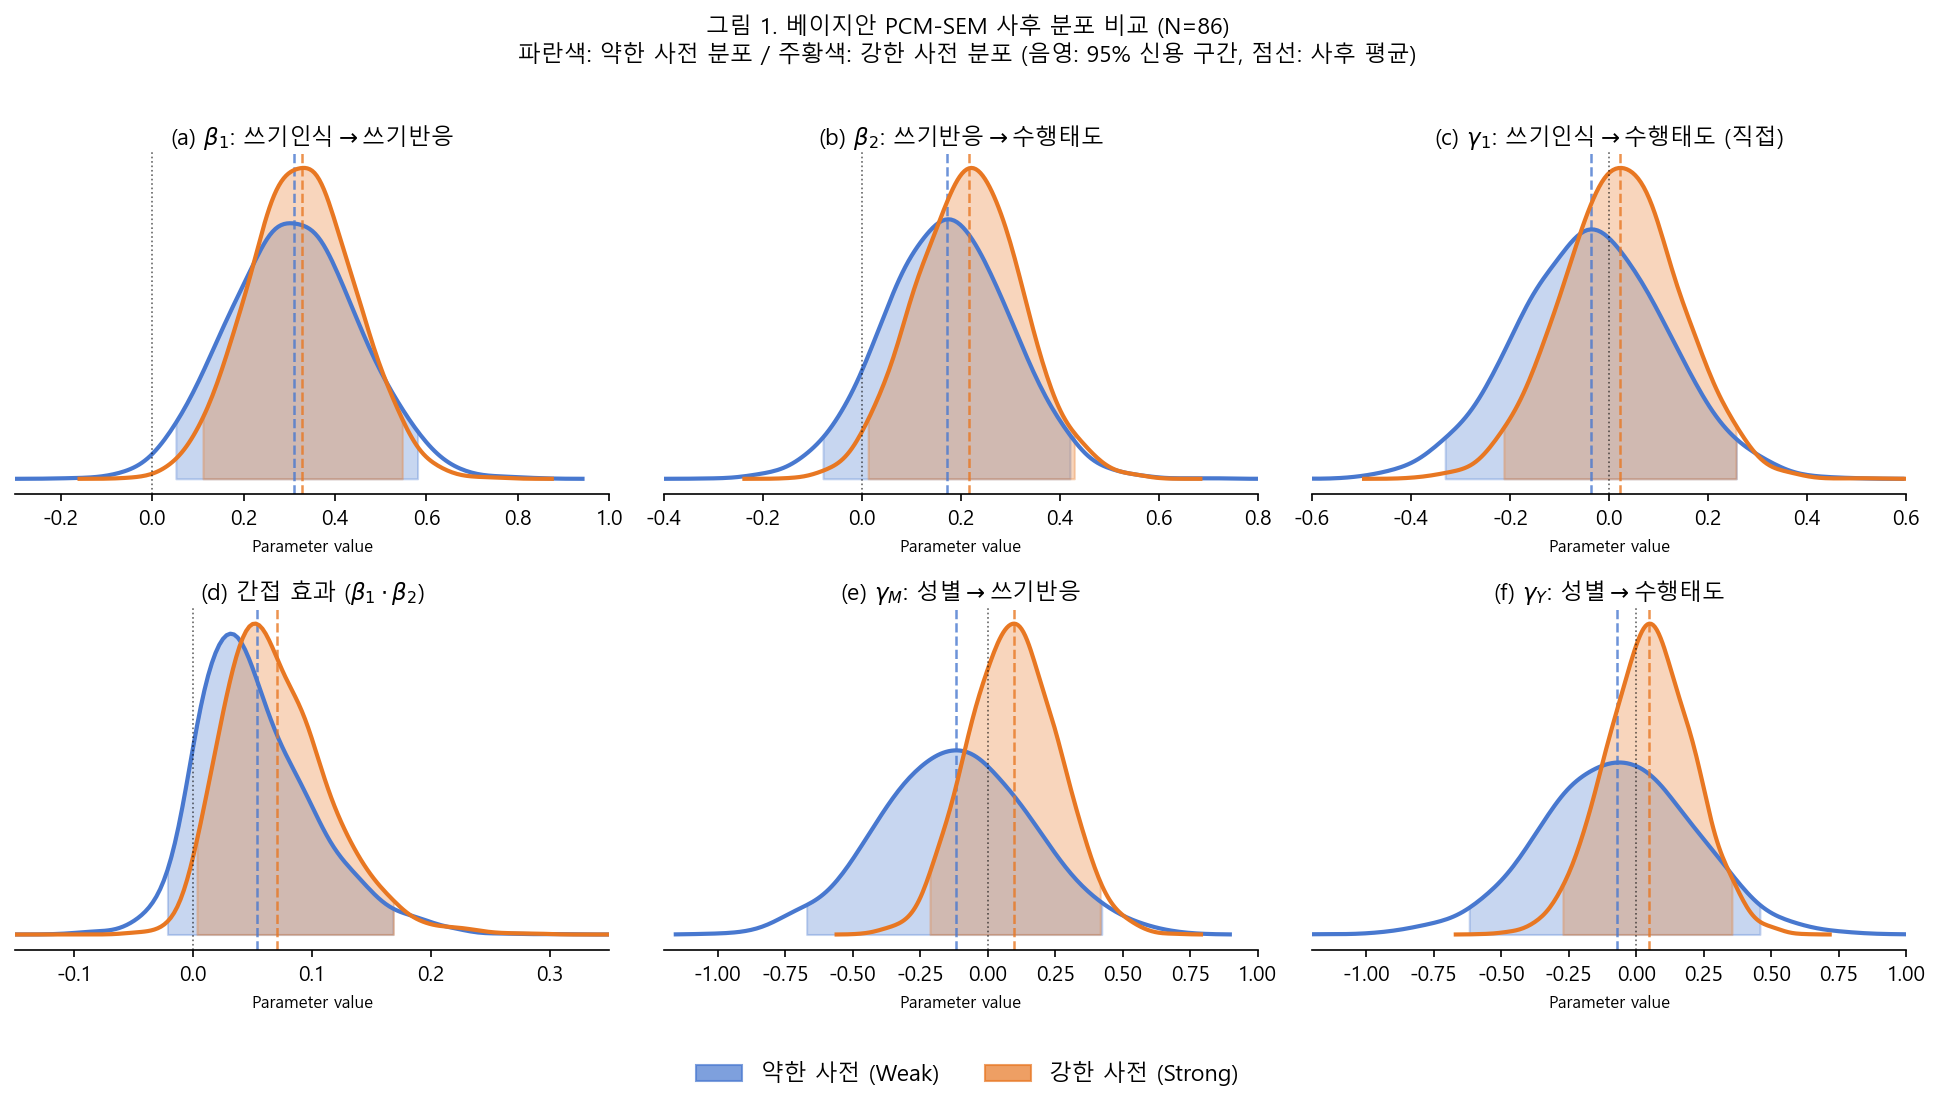
\includegraphics[width=0.92\textwidth]{ss_fig_posterior_combined}
\caption{그림 2. 베이지안 PCM-SEM 사후 분포 비교 (N=86). 파란색: 약한 사전 분포, 주황색: 강한 사전 분포. 음영: 95\% 신용 구간.}
\end{figure}

두 모형의 차이는 소표본(N=86)에서 사전 정보가 갖는 역할을 명확히 보여준다:

\begin{enumerate}
  \item \textbf{신용 구간 폭}: 강한 사전 분포 모형이 전반적으로 좁은 구간을 산출한다 ($\beta_1$ SD: 0.140\ensuremath{\rightarrow}0.115; $\beta_2$ SD: 0.128\ensuremath{\rightarrow}0.107).
  \item \textbf{결론의 변화}: $\beta_2$와 간접 효과의 유의성이 약한 사전에서 강한 사전으로 갈수록 명확해진다.
  \item \textbf{성별 효과}: 약한 사전에서 음의 방향(-0.117), 강한 사전에서 양의 방향(+0.096)으로 바뀐다. 이는 원논문 기반 사전 정보가 추정을 이론 방향으로 안정화시킴을 보여준다.
\end{enumerate}

이상의 결과는 N=86의 소표본에서 베이지안 PCM-SEM의 결론이 사전 분포의 선택에 민감할 수 있음을 시사한다. 복수의 사전 분포를 비교하는 민감도 분석이 소표본 연구에서 특히 중요하다.

\subsubsection{4.3 몬테카를로 시뮬레이션: 방법론적 검증}

베이지안 PCM-SEM의 우위를 방법론적으로 정당화하기 위해, 합산 점수 OLS(CS-OLS)와 잠재 변수 오라클 OLS(LV-OLS)를 6,000회 반복으로 비교하였다.


\noindent\textbf{표 2. $\beta_1$ 추정 성능: 중간 효과 시나리오 (진값 = 0.50)}


\begin{table}[htbp]
\centering
\small
\begin{tabular}{lrrrr}
\toprule
$N$ & CS-OLS 편향 & LV-OLS 편향 & CS-OLS 포함확률 & LV-OLS 포함확률 \\
\midrule
50 & -0.122 & -0.010 & 0.872 & 0.962 \\
86 & -0.109 & 0.000 & 0.840 & 0.944 \\
100 & -0.116 & +0.001 & 0.806 & 0.968 \\
150 & -0.116 & +0.001 & 0.716 & 0.948 \\
200 & -0.115 & 0.000 & 0.670 & 0.946 \\
300 & -0.118 & 0.000 & 0.476 & 0.942 \\
\bottomrule
\end{tabular}
\end{table}

\begin{figure}[htbp]
\centering
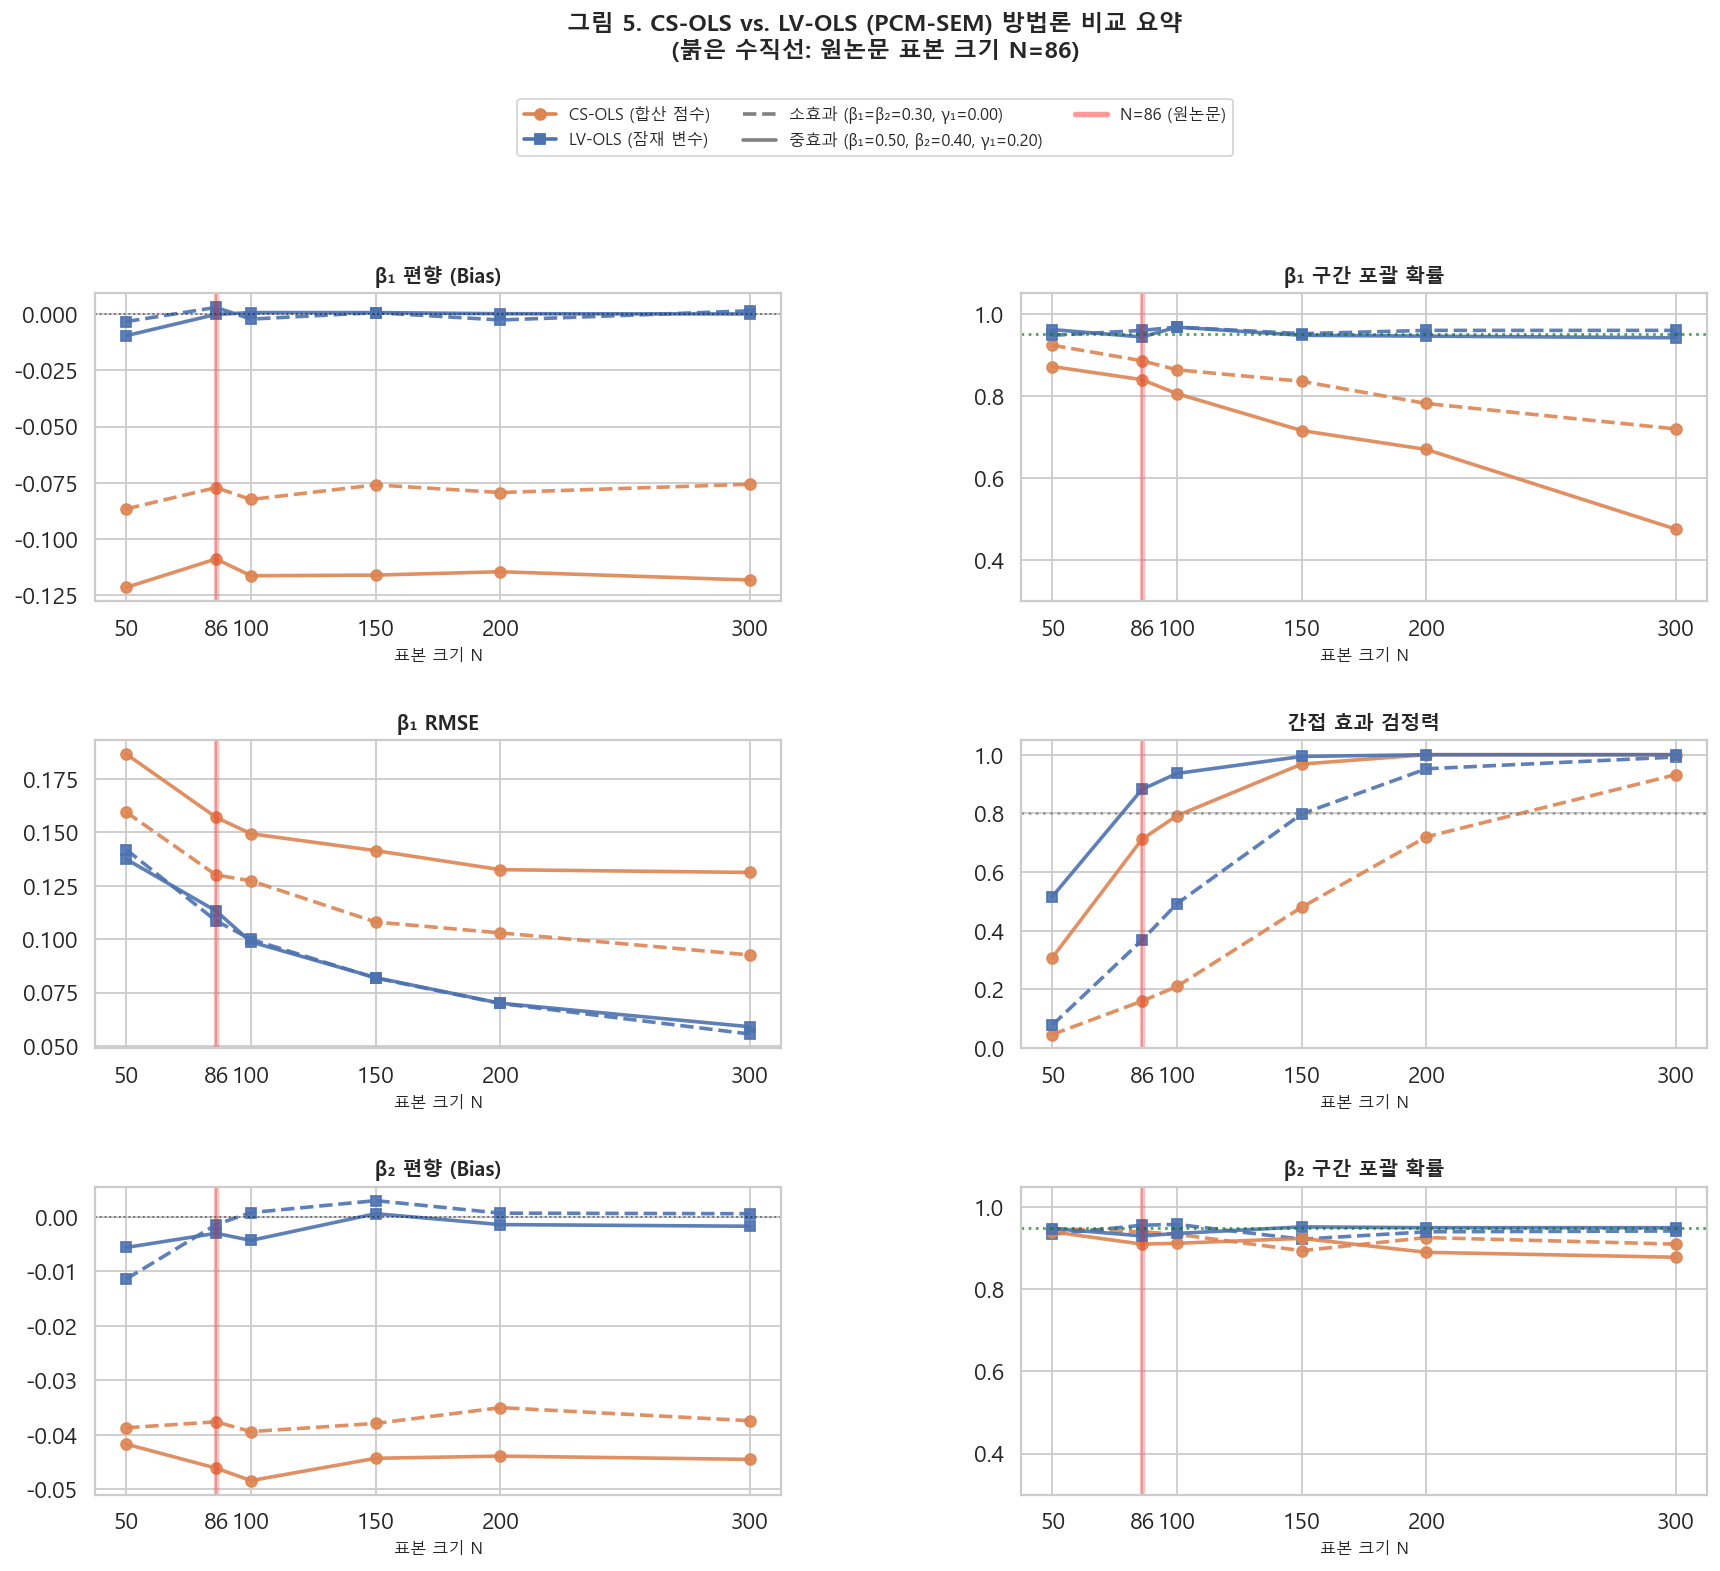
\includegraphics[width=0.92\textwidth]{ss_fig_combined}
\caption{그림 3. CS-OLS vs. LV-OLS(PCM-SEM 이론 상한) 성능 비교. N=86 수직선 기준 LV-OLS 대비 CS-OLS의 편향\ensuremath{\cdot}포함확률 저하가 명확하다.}
\end{figure}

CS-OLS의 편향은 표본 크기에 무관하게 약 -0.11\~{}-0.12로 수렴하며, 포함 확률은 N=300에서 0.476까지 단조 감소한다. LV-OLS는 모든 조건에서 편향 \ensuremath{\approx} 0, 포함 확률 \ensuremath{\approx} 0.95를 유지한다.


\noindent\textbf{표 3. 간접 효과 검출력: 중간 효과 시나리오 ($\beta_1\beta_2 = 0.20$)}


\begin{table}[htbp]
\centering
\small
\begin{tabular}{lrrr}
\toprule
$N$ & CS-OLS 검출력 & LV-OLS 검출력 & 차이 \\
\midrule
50 & 0.308 & 0.516 & +0.208 \\
\textbf{86} & \textbf{0.712} & \textbf{0.882} & \textbf{+0.170} \\
100 & 0.792 & 0.936 & +0.144 \\
150 & 0.968 & 0.994 & +0.026 \\
\bottomrule
\end{tabular}
\end{table}

원논문의 표본 크기(N=86)에서 간접 효과 검출력이 CS-OLS 0.712에서 LV-OLS 0.882로 약 17\%p 향상된다. PCM-SEM이 잠재 변수를 측정 오차 없이 추정한다면 LV-OLS에 근접하므로, 동일 N=86에서 약 17\%p의 검출력 향상이 기대된다.


\section{5. 논의}

\subsubsection{5.1 원논문과의 비교}

원논문(주월랑, 2022)은 세 하위 구인의 기술통계와 집단 차이 분석만을 수행하였다. 본 연구의 PCM-SEM은 다음 세 가지를 추가로 규명하였다.

\textbf{첫째, 인과 매개 구조의 규명.} 쓰기인식\ensuremath{\rightarrow}쓰기반응\ensuremath{\rightarrow}수행태도의 완전 매개(full mediation) 경로가 지지되었다. 직접 효과($\gamma_1 \approx 0$, 두 모형 모두 비유의)는 쓰기인식이 수행태도에 미치는 영향이 \textbf{쓰기반응이라는 정의적 징검다리를 반드시 통과해야만} 전달됨을 의미한다.

이 결과는 원논문(주월랑, 2022)의 핵심 결론인 "정의적 요인 함양에 대한 관심이 필요하다"는 제언에 실증적 경로를 제공한다. 원논문은 집단 차이 분석을 통해 정의적 쓰기 태도가 독립적으로 작동함을 관찰하고 이를 교육적 과제로 남겼는데, 본 연구의 PCM-SEM은 그 메커니즘을 구체화한다: \textbf{쓰기의 가치 인식(인지적)을 높여도 수행태도는 직접 개선되지 않으며, 쓰기에 대한 흥미와 자신감(정의적)이 함께 형성되어야 비로소 수행태도로 연결된다.} 따라서 한국어 쓰기 교육에서 가치 인식 제고 활동(인지적 개입)은 흥미 유발\ensuremath{\cdot}자신감 강화 활동(정의적 개입)과 반드시 병행되어야 효과적이다. 이는 태도 이론의 인지\ensuremath{\rightarrow}정의\ensuremath{\rightarrow}행동 의도 순차 모형(Ajzen \& Fishbein, 1977)이 외국인 유학생 한국어 쓰기 맥락에서도 유효함을 보이는 최초의 정량적 경로 검증이다.

\textbf{둘째, 성별 효과의 재확인.} 원논문이 성별에 따른 집단 차이가 없다고 보고한 것과 일관되게, 두 PCM-SEM 모형 모두 성별이 쓰기반응과 수행태도에 유의한 영향을 미치지 않음을 확인하였다.

\textbf{셋째, 측정 오차 보정의 효과.} 합산 점수 OLS는 $\beta_1$을 약 0.11\~{}0.12 과소추정하는 반면, PCM-SEM은 편향 없는 추정을 제공한다. 원논문의 분석이 합산 점수를 사용하였다면, 쓰기인식과 쓰기반응 간의 실제 관계가 과소추정되었을 가능성이 있다.

\subsubsection{5.2 사전 정보와 소표본 추론}

$\beta_2$(쓰기반응\ensuremath{\rightarrow}수행태도)의 유의성이 약한 사전과 강한 사전 모형 사이에서 달라지는 결과는 중요한 방법론적 교훈을 제공한다. N=86의 소표본에서 단일 추정 결과에만 의존하는 것은 위험하며, 복수의 사전 분포 하에서 결론의 안정성을 점검하는 민감도 분석이 필수적이다.

강한 사전 분포 모형에서 $\beta_2$가 유의해지는 것은, 쓰기 태도 관련 선행 연구의 전형적 효과 크기(r\ensuremath{\approx}0.30\~{}0.55)가 이 경로의 존재를 지지한다는 사전 지식이 반영된 결과이다. 이는 "사전 분포가 결론을 바꿨다"는 의미가 아니라, "사전 지식을 포함하면 동일 데이터에서 더 정밀한 추정이 가능하다"는 베이지안 추론의 원리를 실증한 것이다.

\subsubsection{5.3 연구의 한계}

\textbf{데이터 한계}: 원논문의 개별 응답 데이터를 사용하지 않았으므로, 실제 데이터에서 나타날 수 있는 분포적 이탈(비정규성, 이분산성 등)이 반영되지 않았다. 또한 문항별 세부 통계(문항 평균, 표준편차, 변별도)가 원논문에 미보고되어 PCM 임계값 보정이 구인 수준 평균에만 의존하였다는 한계가 있다.

\textbf{모형 한계}: 오라클 LV-OLS는 완전 정밀한 PCM 추정의 이론적 상한이다. 실제 PCM-SEM에서는 잠재 변수 추정의 불확실성이 추가되므로, 17\%p의 검출력 향상은 상한값으로 해석해야 한다.

\textbf{외적 타당도}: 13개 국적 출신의 소규모 표본으로부터 얻은 결과를 일반화하는 데 주의가 필요하다. 특히 국적, 한국어 숙달도, 전공 계열 등이 통제되지 않은 혼재 변수로 작용할 수 있다.


\section{6. 결론}

본 연구는 원논문(주월랑, 2022)이 검토하지 않은 쓰기 태도 구인 간의 인과 매개 구조를 베이지안 PCM-SEM으로 규명하고, 방법론적 우위를 몬테카를로 시뮬레이션으로 검증하였다. 주요 결론은 다음과 같다.

\textbf{1. 쓰기인식\ensuremath{\rightarrow}쓰기반응\ensuremath{\rightarrow}수행태도의 완전 매개 구조가 지지된다.} 두 경로 모두 양의 방향으로 유의하며, 직접 효과는 비유의적이다. 쓰기인식이 수행태도에 미치는 영향은 쓰기반응이라는 정의적 징검다리를 통해서만 전달되므로, 인지적 개입과 정의적 개입의 병행이 효과적인 한국어 쓰기 교육의 핵심임이 확인된다.

\textbf{2. 사전 정보가 소표본 추론의 질을 향상시킨다.} N=86에서 원논문 통계 기반의 강한 사전 분포 모형은 쓰기반응\ensuremath{\rightarrow}수행태도 경로($\beta_2$)와 간접 효과를 유의하게 추정하여, 약한 사전 분포 모형보다 명확한 결론을 제공한다. 이는 베이지안 지식 누적의 실증적 효과이다.

\textbf{3. 합산 점수 OLS는 체계적 편향을 유발한다.} N=86에서 $\beta_1$ 편향은 약 \ensuremath{-}0.11이며, 간접 효과 검출력이 PCM-SEM 대비 17\%p 낮다. 표본이 커질수록 포함 확률이 오히려 악화된다.

\textbf{4. 베이지안 PCM-SEM은 빈도주의 방법이 제공하지 못하는 확률적 추론을 가능하게 한다.} 인과 방향성 확률($\approx 91\text{~}98\%$), 간접 효과의 완전한 사후 분포, 매개 가설에 대한 직접적 확률 계산이 가능하다. 발산 전이 0건, $\hat{R} \leq 1.001$, ESS \ensuremath{\geq} 3,333으로 모든 추론이 수치적으로 안정된 샘플에 기반함이 확인되었다.

향후 연구에서는 실제 설문 응답 데이터를 수집하여 문항 수준 진단(PCM 문항 적합도, 개인-문항 지도)을 포함한 완전한 PCM-SEM 분석을 수행할 필요가 있다.


\section*{참고문헌}
\begin{hangparas}{1em}{1}
Ajzen, I., \& Fishbein, M. (1977). Attitude-behavior relations: A theoretical analysis and review of empirical research. \textit{Psychological Bulletin}, \textit{84}(5), 888–918.

Bernardo, J. M., \& Smith, A. F. M. (1994). \textit{Bayesian theory}. Wiley.

Bandura, A. (1977). Self-efficacy: Toward a unifying theory of behavioral change. \textit{Psychological Review}, \textit{84}(2), 191–215.

Carpenter, B., Gelman, A., Hoffman, M. D., Lee, D., Goodrich, B., Betancourt, M., ... \& Riddell, A. (2017). Stan: A probabilistic programming language. \textit{Journal of Statistical Software}, \textit{76}(1), 1–32.

Fuller, W. A. (1987). \textit{Measurement error models}. Wiley.

Gelman, A., \& Rubin, D. B. (1992). Inference from iterative simulation using multiple sequences. \textit{Statistical Science}, \textit{7}(4), 457–472.

Hedges, L. V., \& Olkin, I. (1985). \textit{Statistical methods for meta-analysis}. Academic Press.

Hoffman, M. D., \& Gelman, A. (2014). The No-U-Turn sampler. \textit{Journal of Machine Learning Research}, \textit{15}, 1593–1623.

Masters, G. N. (1982). A Rasch model for partial credit scoring. \textit{Psychometrika}, \textit{47}(2), 149–174.

Muthén, L. K., \& Muthén, B. O. (2002). How to use a Monte Carlo study to decide on sample size and determine power. \textit{Structural Equation Modeling}, \textit{9}(4), 599–620.

Sobel, M. E. (1982). Asymptotic confidence intervals for indirect effects in structural equation models. \textit{Sociological Methodology}, \textit{13}, 290–312.

Spearman, C. (1904). The proof and measurement of association between two things. \textit{American Journal of Psychology}, \textit{15}(1), 72–101.

주월랑 (2022). 학문 목적 한국어 학습자의 한국어 쓰기 태도 연구. \textit{반교어문연구}, 제63집, pp. 185-208.
\end{hangparas}

\section{부록 A. 소프트웨어 및 재현 가능성}

모든 분석은 Python 3.12(numpy 1.24, pandas 2.0), cmdstanpy 1.3.0, CmdStan 2.33 이상으로 수행되었다. 난수 시드 2024. 소스 코드:

\begin{table}[htbp]
\centering
\small
\begin{tabular}{lr}
\toprule
파일 & 내용 \\
\midrule
\texttt{sem\_pcm\_v2.stan} & 약한 사전 분포 PCM-SEM Stan 모형 \\
\texttt{sem\_pcm\_with\_prior.stan} & 강한 사전 분포 PCM-SEM Stan 모형 \\
\texttt{ss\_run\_with\_prior.py} & 베이지안 MCMC 실행 (두 모형 비교) \\
\texttt{ss\_monte\_carlo.py} & Monte Carlo 시뮬레이션 엔진 \\
\texttt{ss\_results.csv} & Monte Carlo 원시 결과 (6,000행) \\
\texttt{ss\_mcmc\_weakprior\_N86.csv} & 약한 사전 MCMC 샘플 \\
\texttt{ss\_mcmc\_strongprior\_N86.csv} & 강한 사전 MCMC 샘플 \\
\texttt{ss\_fig\_posterior.py} & MCMC 사후 분포 시각화 (그림 2) \\
\bottomrule
\end{tabular}
\end{table}

\section{부록 B. 소 시나리오 Monte Carlo 결과}


\noindent\textbf{표 B1. $\beta_1$ 성능: 소 효과 시나리오 (진값 = 0.30)}


\begin{table}[htbp]
\centering
\small
\begin{tabular}{lrrrr}
\toprule
$N$ & CS-OLS 편향 & LV-OLS 편향 & CS-OLS 포함확률 & LV-OLS 포함확률 \\
\midrule
50 & -0.087 & -0.003 & 0.924 & 0.948 \\
86 & -0.077 & 0.003 & 0.886 & 0.960 \\
150 & -0.076 & 0.001 & 0.836 & 0.952 \\
300 & -0.076 & 0.002 & 0.720 & 0.960 \\
\bottomrule
\end{tabular}
\end{table}

CS-OLS = 합성점수 최소제곱법; LV-OLS = 잠재변수 OLS(오라클); 포함확률 = 95\% CI가 진값을 포함한 비율.
소 효과 시나리오에서도 CS-OLS의 하향 편향(약 \ensuremath{-}0.08)은 표본크기와 무관하게 지속되며, 포함확률은 N=300에서 0.72로 하락하여 심각한 1종 오류 왜곡을 나타낸다.
\end{document}
